\documentclass{article}
\usepackage{amsmath, amssymb, graphicx, hyperref}

\title{Hamilton-Jacobi Reachability}
\author{}
\date{}

\begin{document}

\maketitle


\section{Motivations!}
We want \textit{value functions} for safety control. Those can be certificates. Take some desired safety constraint, and the long-term effects of the dynamics, and convert it into a single scalar function. Recall my first presentation on CBF, and the diagram. 

Note that ``Levels'' indicate the measure of the safety margin, and the gradient demonstrates the direction. 

What I want to do in this quick talk is to combine both ideas of HJR and CBF, It helps me because my research atm is leveraging HJR into CBF definitions of my control, (based on ideas in Safe-Diffuser), and also I want to teach this idea someday. 

\section{Key ideas}
If you get nothing else from this, Offline: HJR finds the safety value function. Online, HJR uses that safety value function for safe control.

\section{HJR Offline}
Consider a dynamical system $\dot z = f(z, u, d)$ where $z$ is state, $u$ is control, $d$ is disturbance. We usually think of disturbances as bounded, but in the case of my research, I'm going to think of them as stochastic. For this, though, call them bounded.

Reachability is just brute-force DP.

\subsection{Reachability problems}
We have sets vs tubes. A set is like asking what are the set of states where I would inevitably given some time $t$ something happens? Herbert uses a tree analogy.

Tube is slightly different, it considers \textit{within} some time $t$, 

Avoid versus reach:
Avoid means to avoid a set, reach means to reach a set.

Finite time vs infinite time: In infinite time, avoid converges. There is usually a path to avoid. Reach generally doesn't. 

Backwards vs forward reachability.

Backwards means looking at the backwards destination and then looking in time, while forwards means looking at initial state, and then seeing all the places I can reach in some time. 

Now consider the infinite time case. How do you avoid something in some infinite time horizon?

\subsection{Example}
Consider an Infinite time Avoid BRS with the following parameters:

\[\dot x = v_x \] 
\[\dot v_x = u \] 
\[ u \in [-1, 1] \]

We also have some obstacle from $-1 \leq x \leq 1$. 

First graph shows this. 
\begin{figure}[h!]
    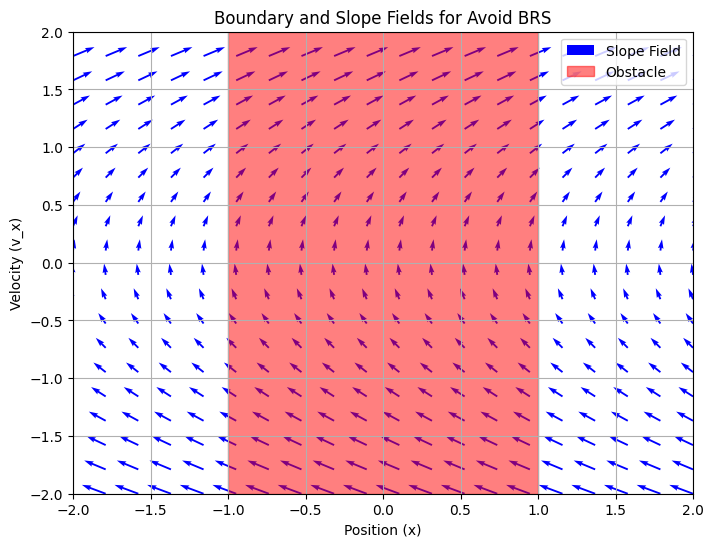
\includegraphics[width = \textwidth]{screenshot11oct1.png}
\end{figure}


Now we definine a terminal cost function, defined as like distance to the obstacle. 

My graph looks terrible, but I'll come back to it. 

Edit: I ended up stealing the image from Sylvia Herbert for this:
\begin{figure}[h!]
    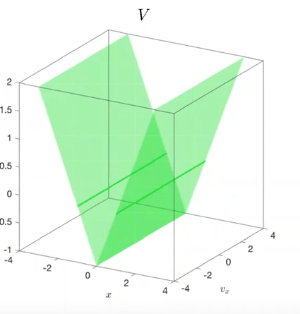
\includegraphics[width = \textwidth]{Screenshot 2024-10-11 125926.png}
\end{figure}


To calculate the Backwards Reachable Set, we calculate the \textit{Hamilton-Jacobi Isaacs Equation}, defined as follows: 

\[ \frac{dV}{dt} + \max_u \langle f(x,u), \nabla V \rangle = 0 \]
This is essentially saying maximize along the gradients, while also saying obey the system dynamics. 

Here, left of the boundary $\frac{dV}{dx} = -1$, $\frac{dV}{dV_x} = 0$, and right of the boundary $\frac{dV}{dx} = 1$, $\frac{dV}{dV_x} = 0$.

So, we are solving the following:

\[\frac{-dV}{dt} = \max_u \{\frac{dV}{dx}\frac{dx}{dt} + \frac{dV}{dVx}\frac{dv_x}{dt}\} \]
Plugging in everything (input arguments, chain rule, etc), we get an update equation of 
\[\frac{-dV}{dt} = \frac{dV}{dx}v_x + \vert \frac{dV}{dV_x} \vert \]

TLDR: Encode the safety constraint into the construction of the value function, then add DP. 


In reachability, we have a \textit{Least-restrictive control law}. That is, switch to the reachable control law only when you are close to the boundary. 

\section{Level Set Approach}
The level set method is commonly used to solve the HJI PDE. The key idea is to represent the target set \(G_0\) as the zero sublevel set of a Lipschitz function \(g(x)\), i.e., \(x \in G_0 \iff g(x) \leq 0\). The BRS can be computed as:
\[
G(t) = \{ x \mid G(t, x) \leq 0 \}
\]
where \(G(t,x)\) satisfies the HJI PDE:
\[
\frac{\partial G(t,x)}{\partial t} + H(t,x, \nabla G(t,x)) = 0, \quad G(0,x) = g(x)
\]
This method transforms the reachability problem into a computationally tractable PDE-solving process.

\section{Forward vs. Backward Reachable Sets}
In addition to backward reachable sets (BRS), forward reachable sets (FRS) can also be computed. The FRS represents all states that can be reached from a given initial set of states after a time duration \(|t|\). Formally:
\[
W(t) = \{ y \mid \exists \gamma \in \Gamma(t), \forall a(\cdot) \in A, \ \zeta(t; x, 0, a(\cdot), \gamma[a](\cdot)) = y, \ x \in G_0 \}
\]
The FRS is useful in different contexts, such as planning the reachable future states of a system.

\section{Reachable Tubes}
The reachable set defined above only includes states that can reach the target at exactly the terminal time. In contrast, reachable tubes capture states that can reach the target within a time duration:
\[
G(t) = \{ x \mid \exists \gamma \in \Gamma(t), \forall a(\cdot) \in A, \ \exists s \in [t,0], \ \zeta(s;x,t,a(\cdot),\gamma[a](\cdot)) \in G_0 \}
\]
This is particularly useful for safety analysis, where we care about avoiding the target set at any time during the horizon.

\section{Two-Player Zero-Sum Differential Games}
In the context of reachability, we often model the problem as a two-player zero-sum game between the controller and disturbance. The objective of the controller is to maximize the outcome (avoid the target), while the disturbance aims to minimize it (drive the system into the target). The cost function over a time horizon \([t,0]\) is given by:
\[
J_t(x, a(\cdot), b(\cdot)) = \int_t^0 c(x(s), a(s), b(s), s) \, ds + q(x(0))
\]
The value function is:
\[
G(t,x) = \inf_{\gamma \in \Gamma(t)} \sup_{a(\cdot) \in A} J_t(x, a(\cdot), \gamma[a](\cdot))
\]
Solving this optimization problem gives the optimal strategies for both players.

\section{Computational Tools}
Two popular computational tools for solving HJ reachability problems are:
\begin{itemize}
    \item \textbf{Level Set Toolbox (toolboxLS)}: A MATLAB toolbox for solving HJ PDEs using level set methods.
    \item \textbf{BEACLS Toolbox}: A C++ toolbox that uses GPU parallelization to accelerate reachability computation.
\end{itemize}


\end{document}
